%%%%%%%%%%%%%%%%%%%%%%%%%%%%%%%%%%%%%%%%%%%%%%%%%%%%%%%%%%%%%%%%%%%%%%%%%%%%%%%%
\section{Supplementary materials}
%%%%%%%%%%%%%%%%%%%%%%%%%%%%%%%%%%%%%%%%%%%%%%%%%%%%%%%%%%%%%%%%%%%%%%%%%%%%%%%%

\begin{figure}[!htbp]
  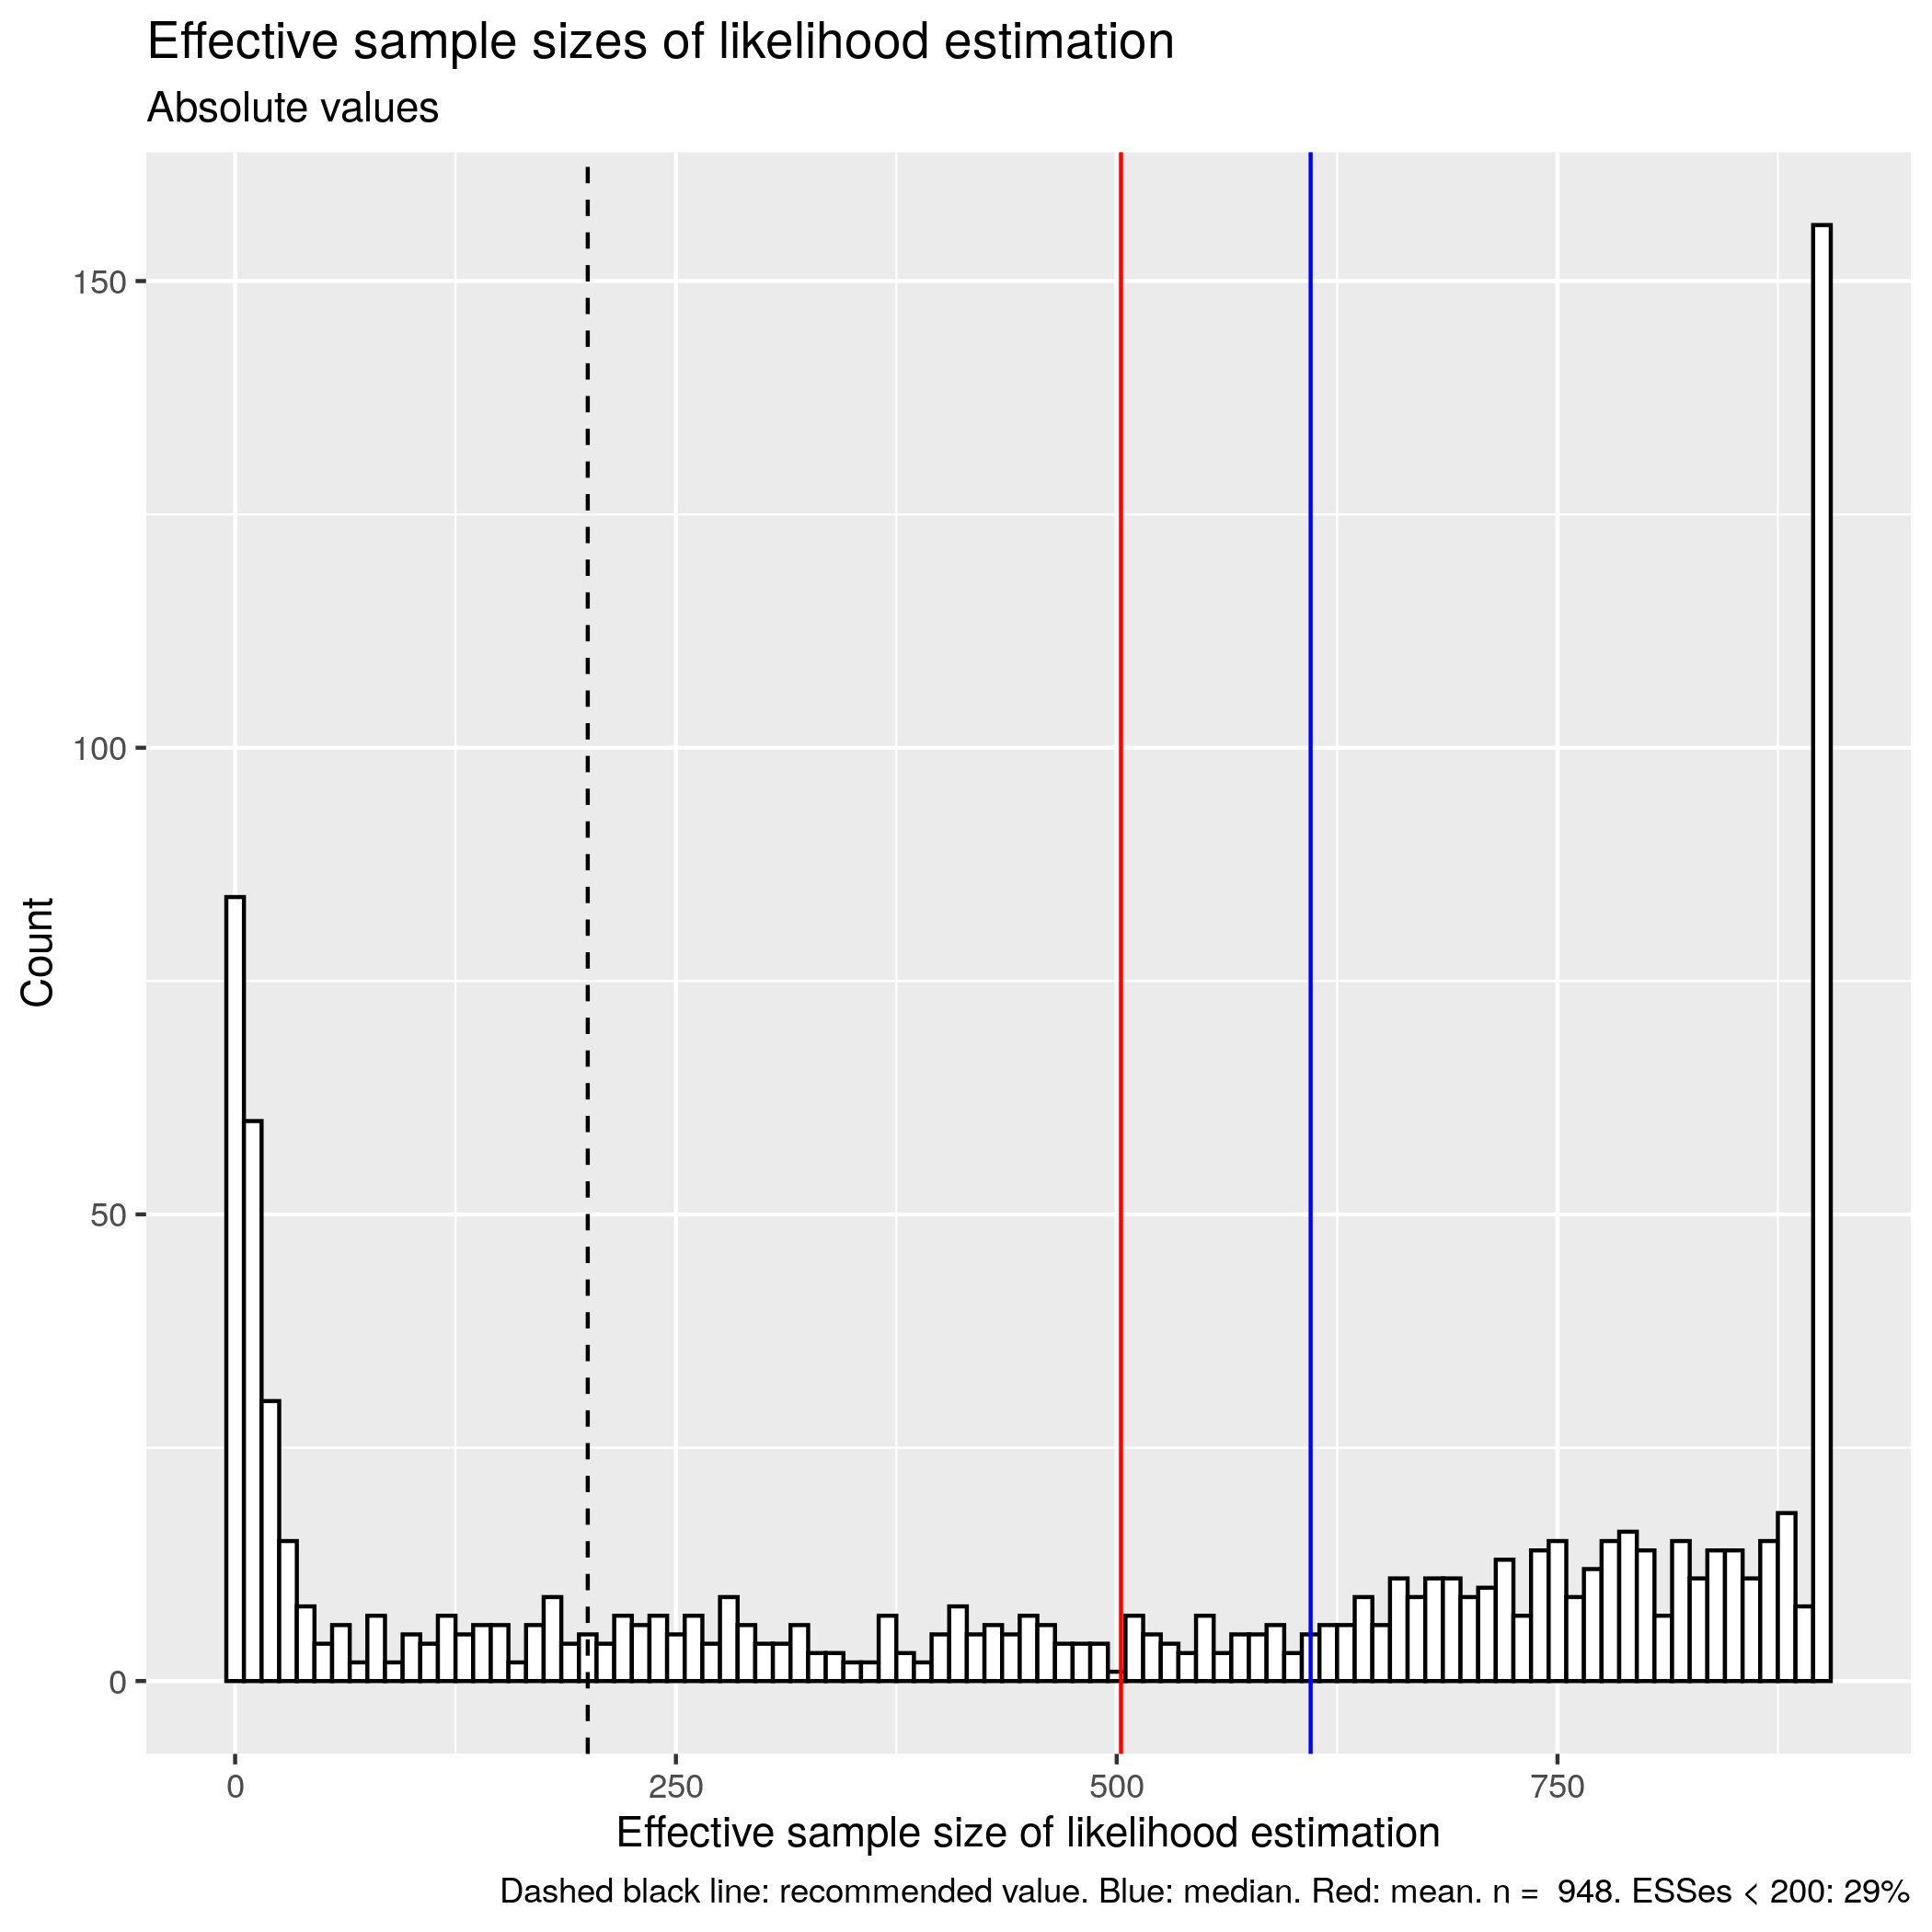
\includegraphics[width=\textwidth]{20190905_fig_esses.png}
  \caption{
    Effective sample sizes of the likelihood of all the experiments that
    finished within 10 days. 
    Each point is one parameter setting.
  }
  \label{fig:esses}
\end{figure}

\begin{figure}[!htbp]
  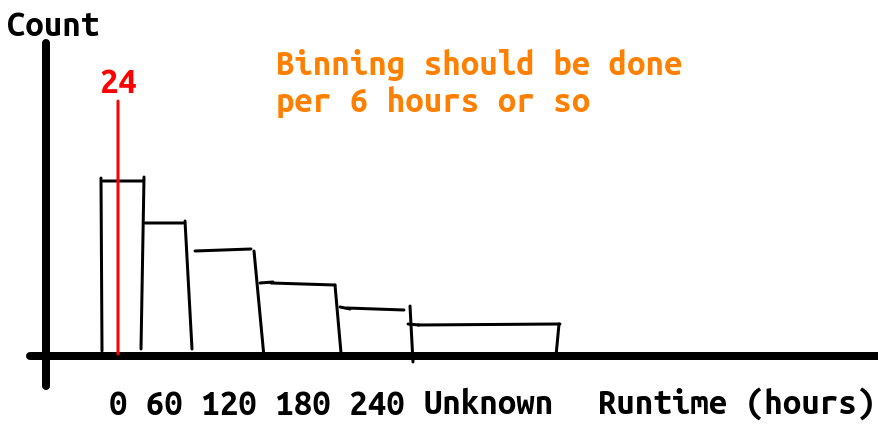
\includegraphics[width=\textwidth]{fig_runtimes.png}
  \caption{
    Distribution of runtimes for all experiments.
    Experiments that did not finish within 10 days end up
    in the 'Unknown' bin.
    Each point is one parameter setting.
    \richel{I suggest:}The vertical line denotes 24 hours. The mean runtime is
    [value], which should be below 24 hours \richel{see my suggestion at
    'parameter settings'}
  }
  \label{fig:runtimes}
\end{figure}

\begin{figure}[!htbp]
  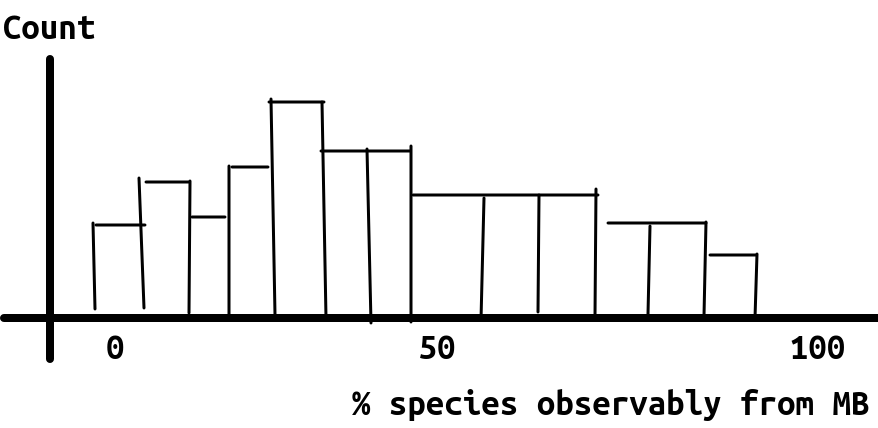
\includegraphics[width=\textwidth]{fig_mbness.png}
  \caption{
    Histogram of the percentage of species that are 
    observably generated in an MB event. 
    Each point corresponds to one true phylogeny.
    Figure \ref{fig:mbness_per_parameter_setting} 
    shows the MBness per parameter setting.
  }
  \label{fig:mbness}
\end{figure}

\begin{figure}[!htbp]
  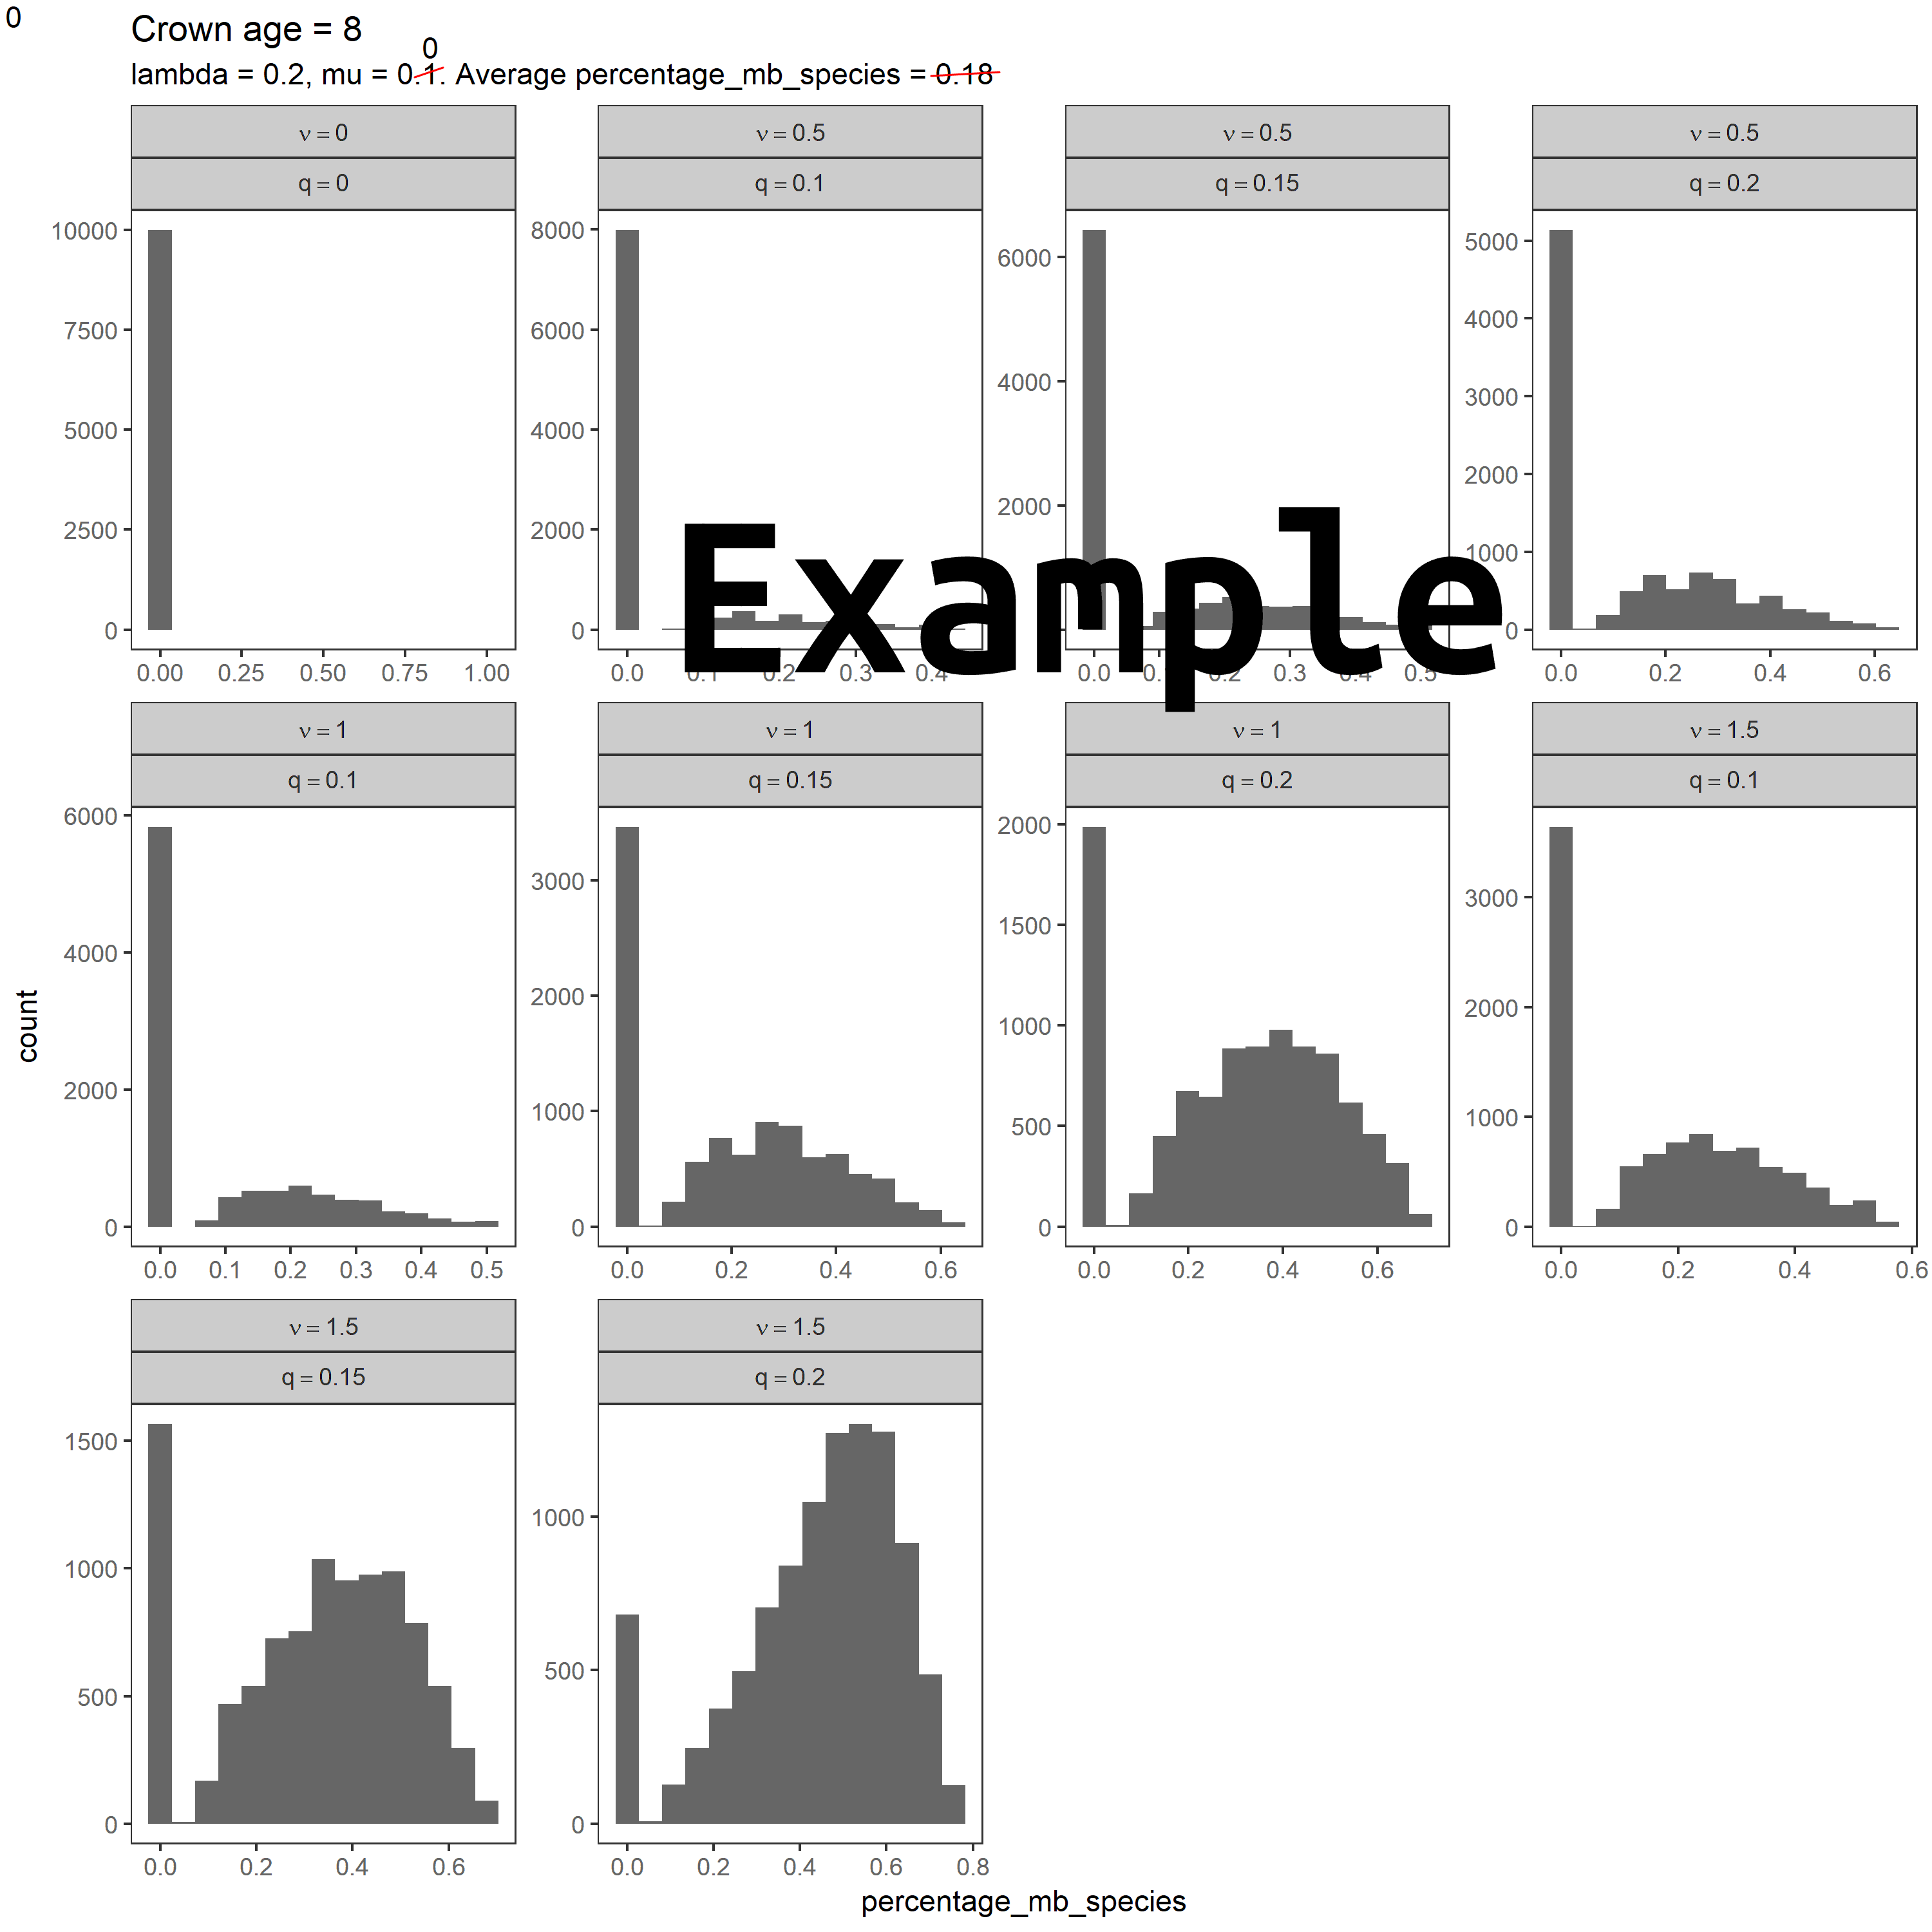
\includegraphics[width=\textwidth]{p_mb_yule.png}
  \caption{
    Histogram of the percentage of species that are 
    observably generated in an MB event, per
    Yule (extinction rate is zero) parameter setting.
    Each point corresponds to one true phylogeny.
  }
  \label{fig:mbness_per_yule_parameter_setting}
\end{figure}

\begin{figure}[!htbp]
  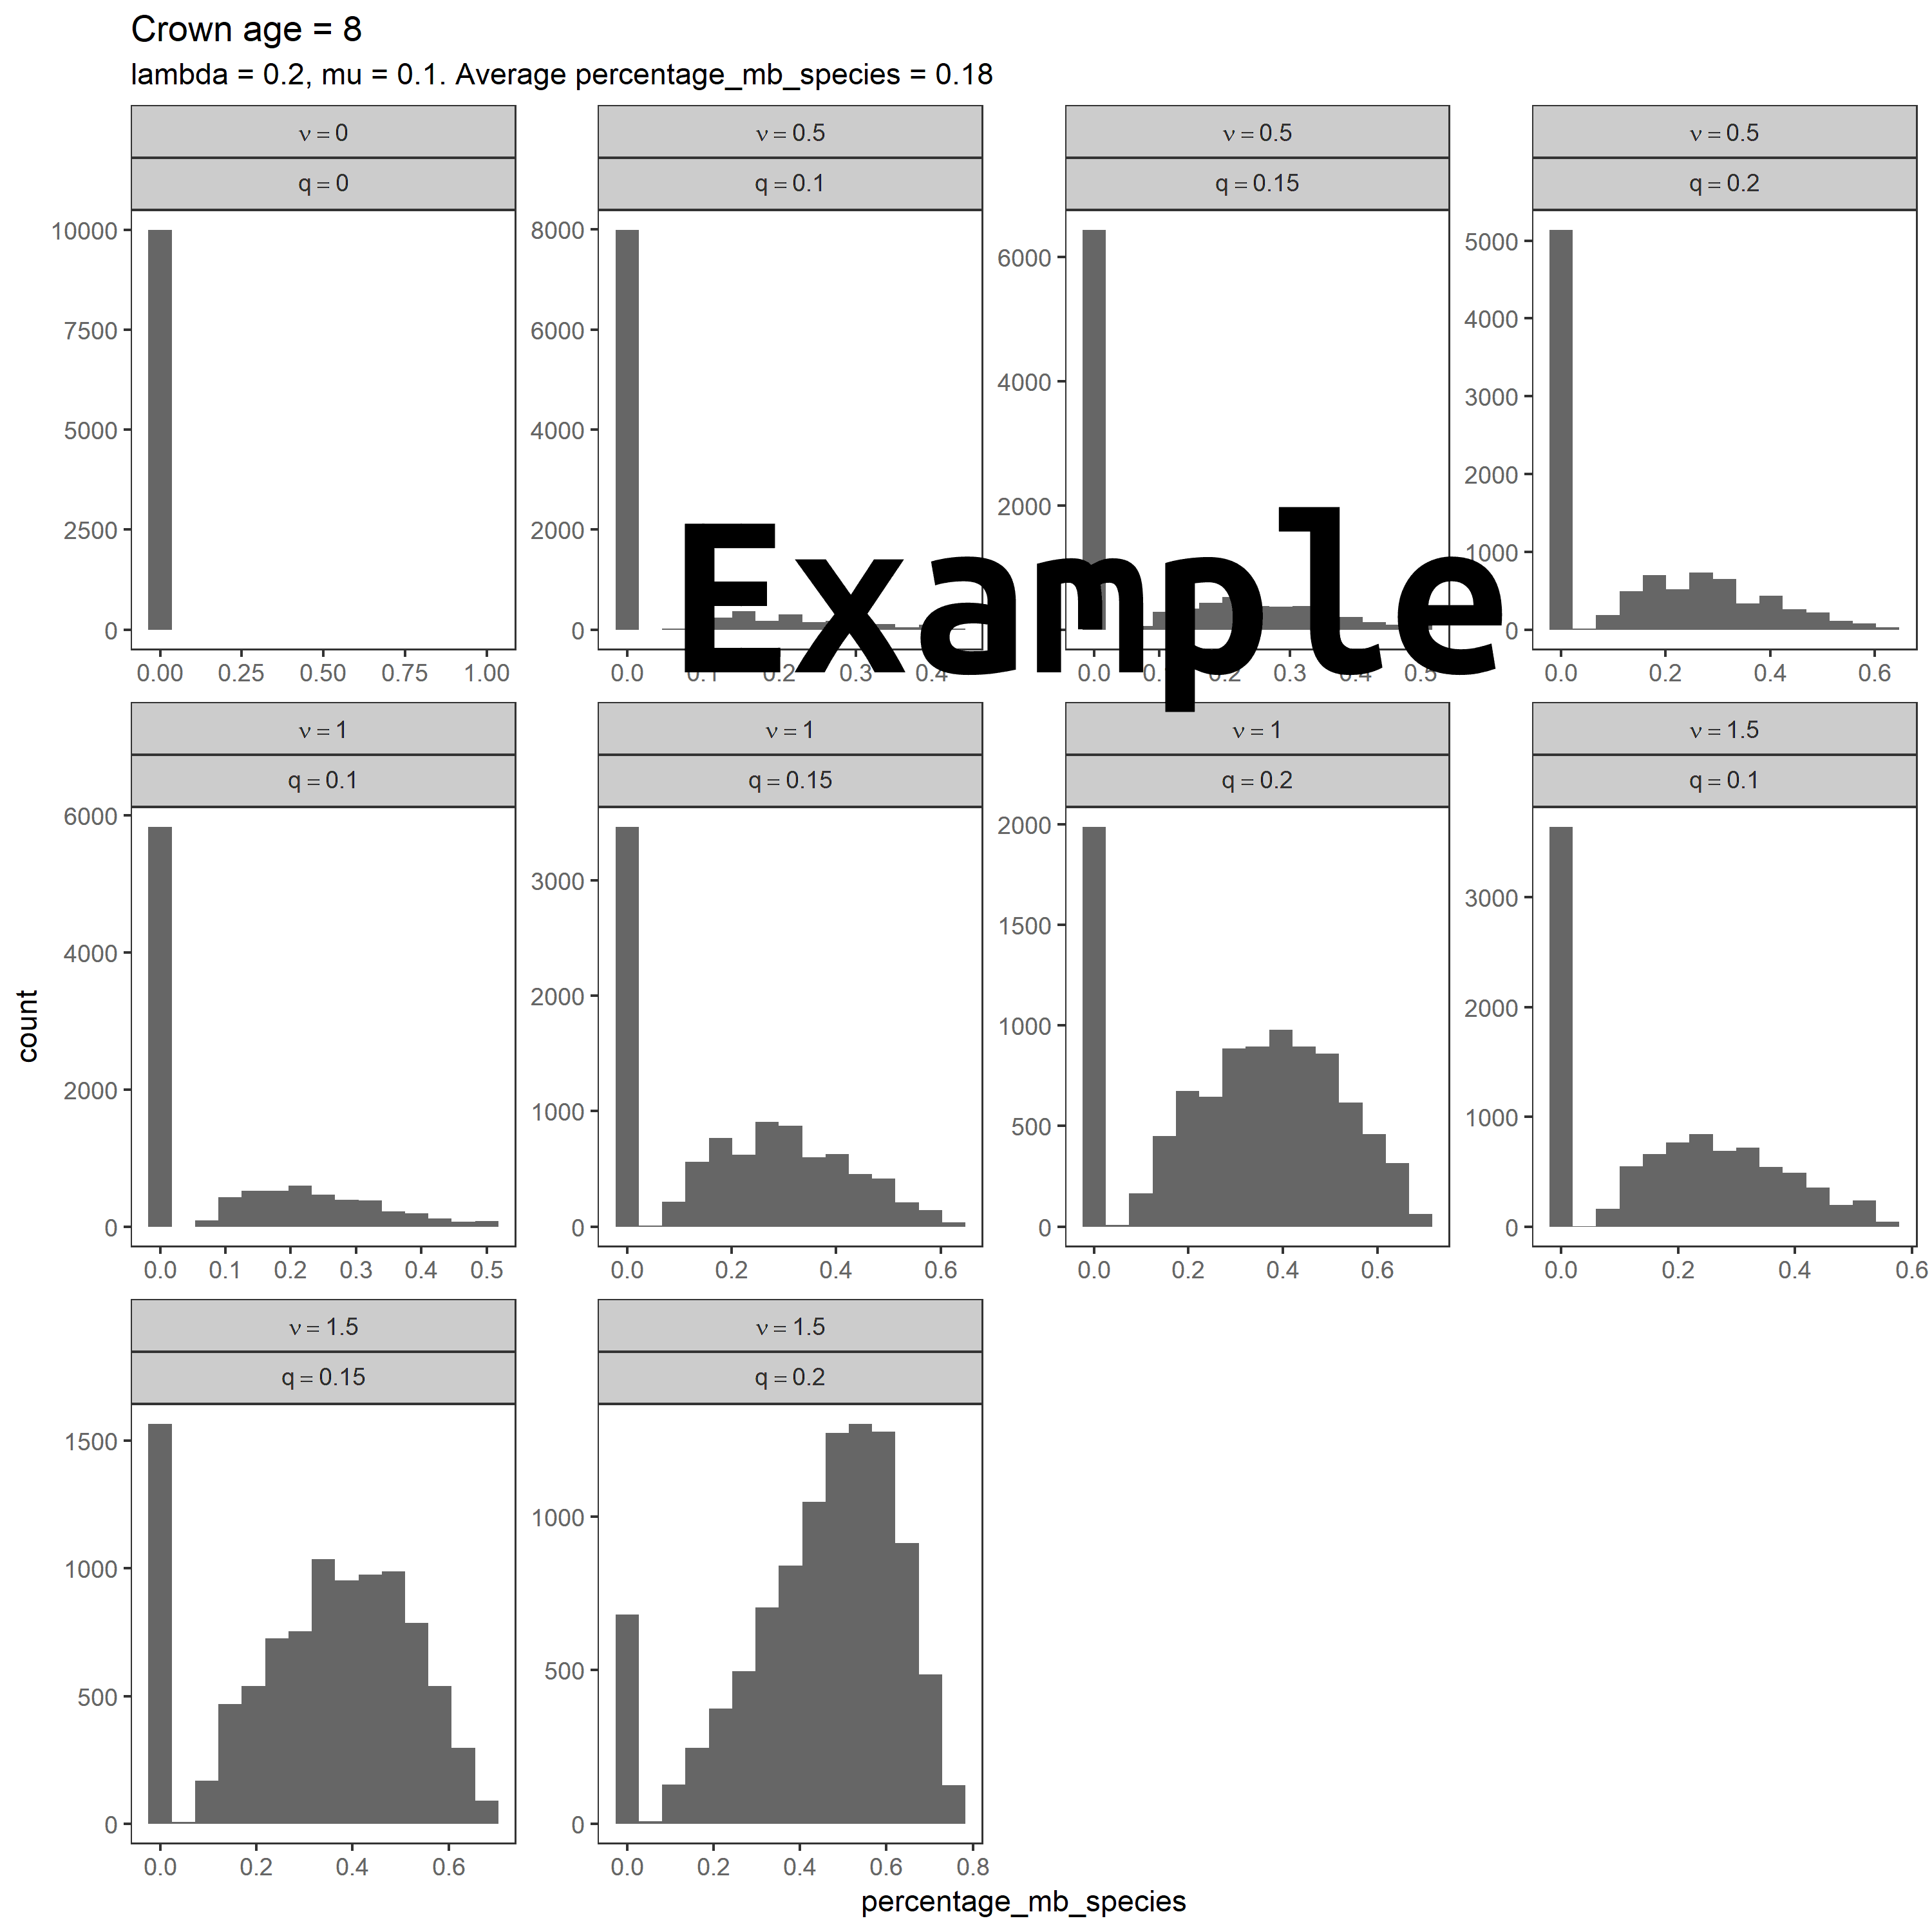
\includegraphics[width=\textwidth]{p_mb_bd.png}
  \caption{
    Histogram of the percentage of species that are 
    observably generated in an MB event, per
    BD (extinction rate is non-zero) parameter setting.
    Each point corresponds to one true phylogeny.
  }
  \label{fig:mbness_per_bd_parameter_setting}
\end{figure}

\begin{figure}[!htbp]
  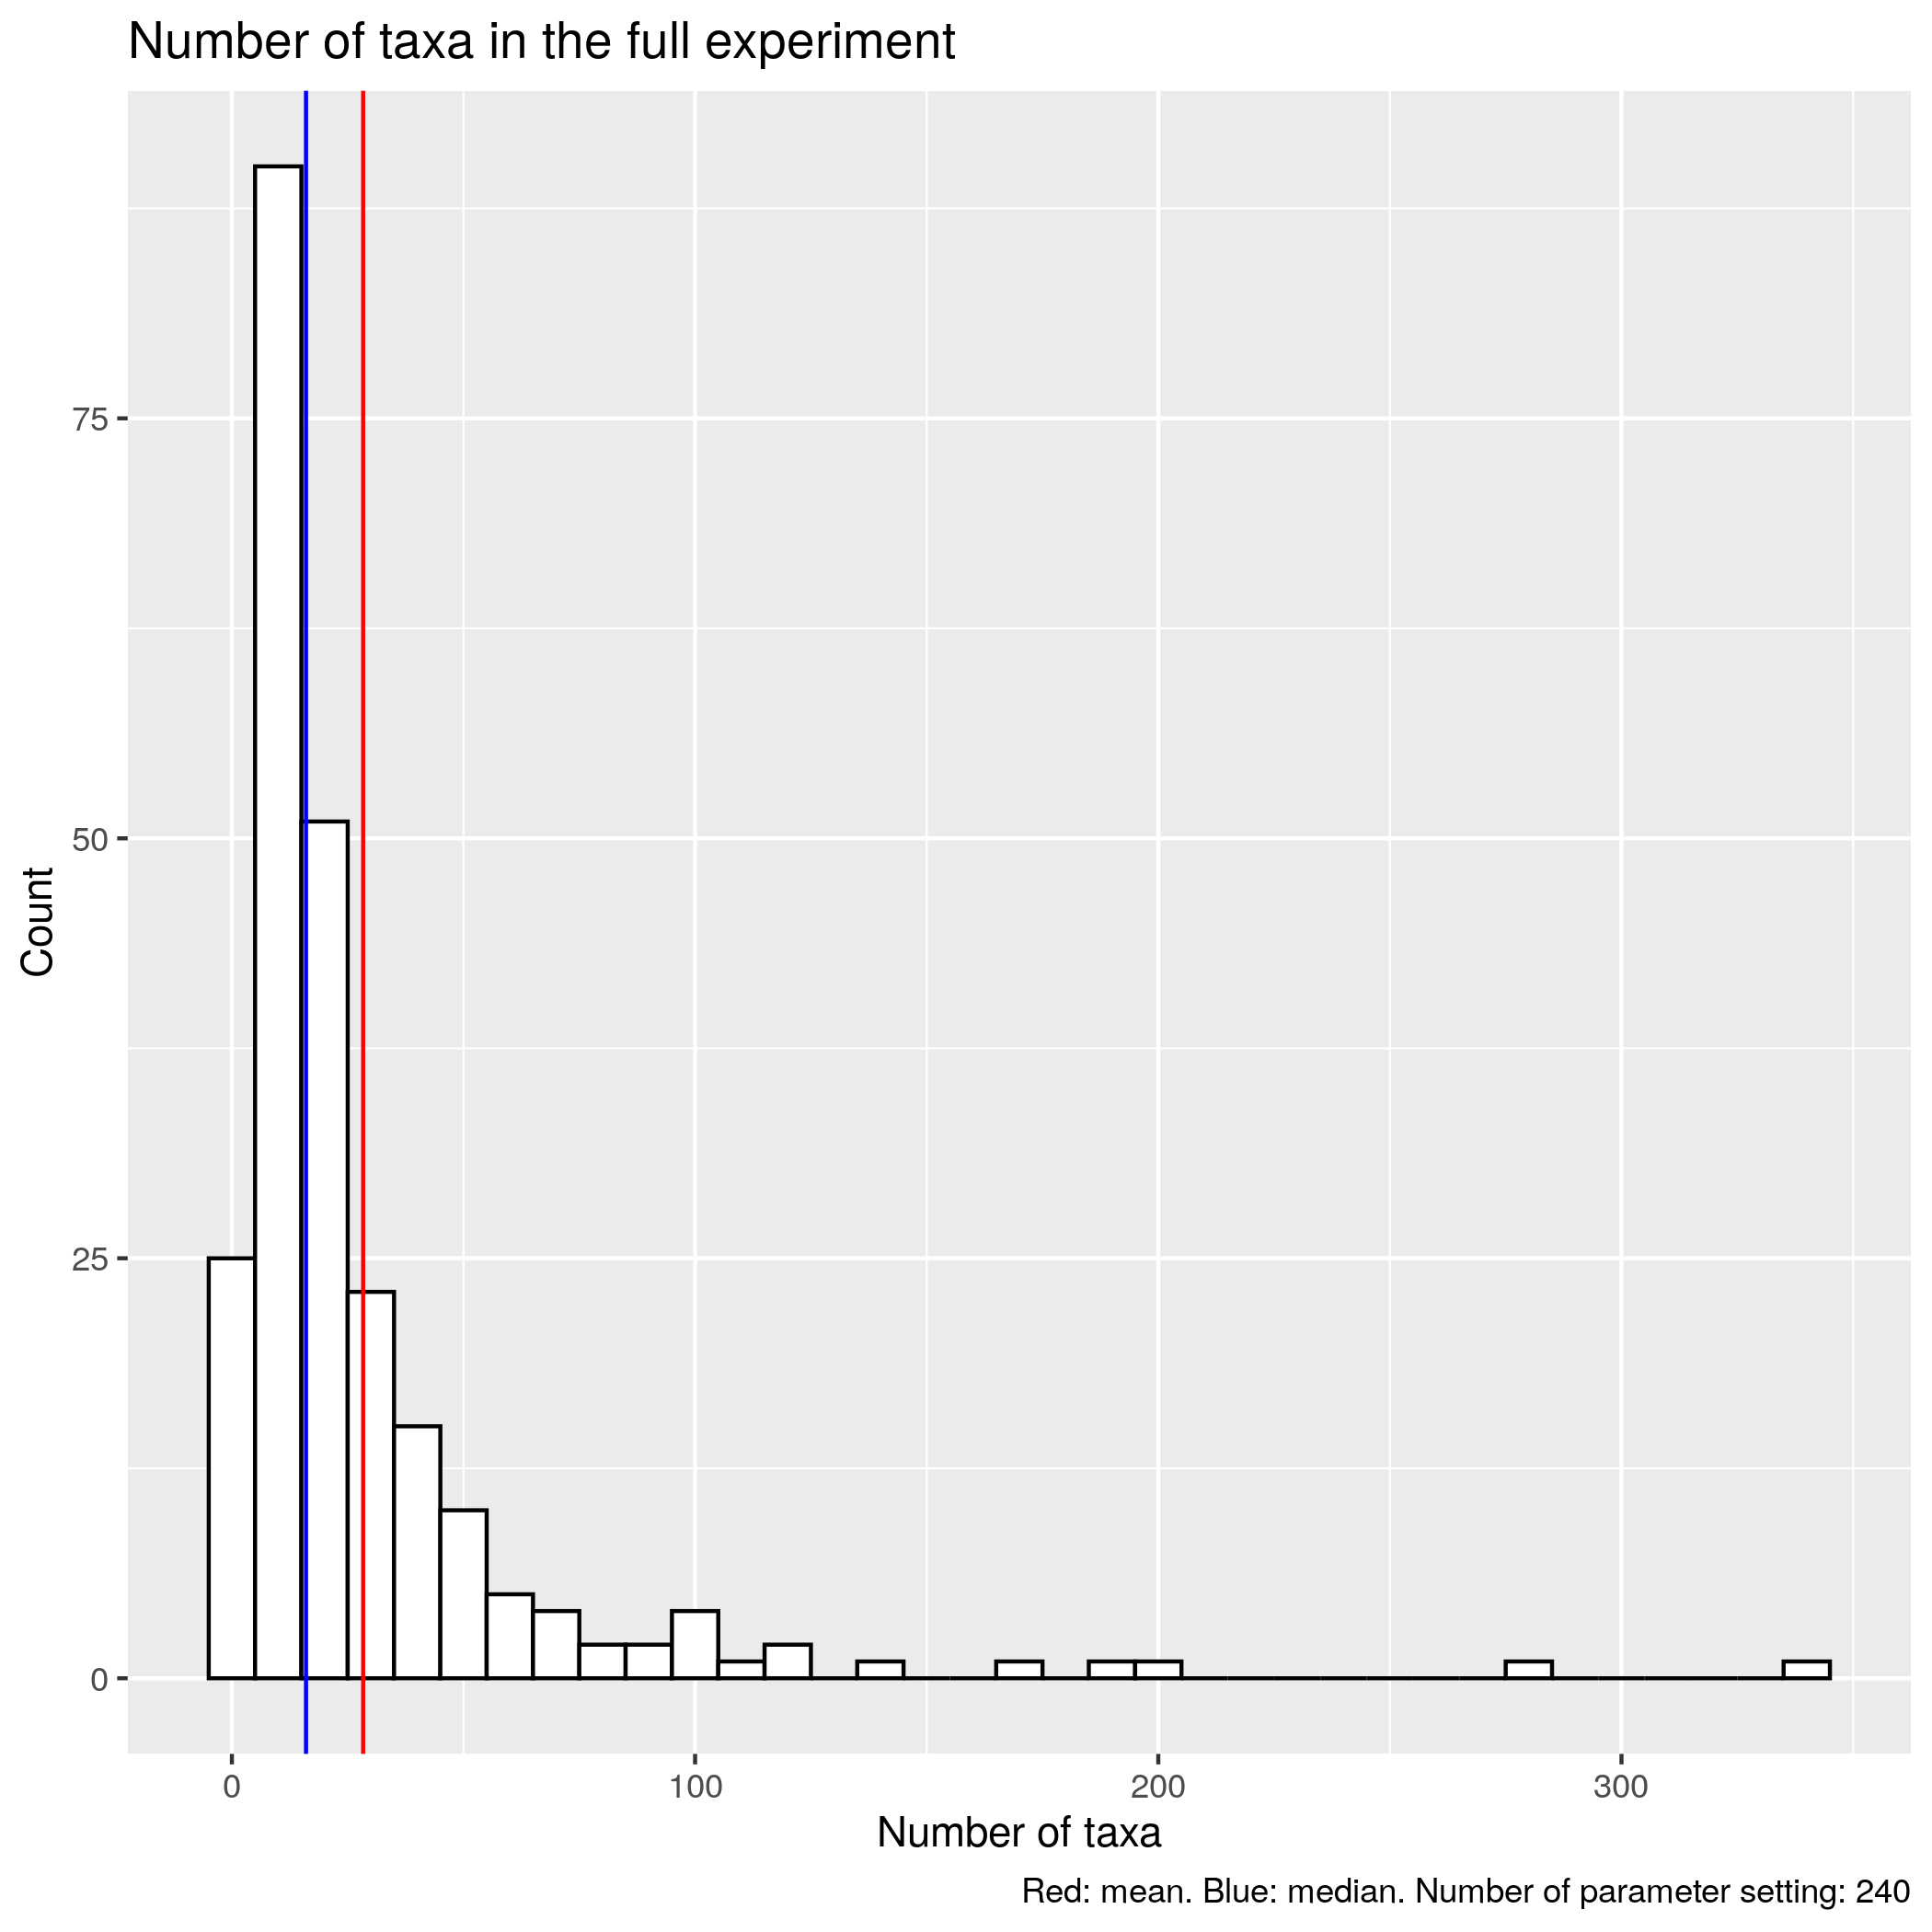
\includegraphics[width=\textwidth]{20190905_fig_n_taxa.png}
  \caption{
    Histogram of the number of taxa in the full experiment.
  }
  \label{fig:n_taxa}
\end{figure}

